%!TEX root = paper.tex
%%%%%%%%%%%%%%%%%%%%%%%%%%%%%%%%%%%%%%%%%%%%%%%%%%%%%%%%%%%%%%%%%%%%%%%%%%%%%%%
\section{Gamer Utility Models}
\label{sec:utilitymodel}

%%%%%%%%%%%%%%%%%%%%%%%%%%%%%%%%%%%%%%%%%%%%%%%%%%%%%%%%%%%%%%%%%%%%%%%%%%%%%%%%
This section now turns to modeling gamer utility as a function
of cost. The model assumes a utility proportional to the number
of games playable, given the amount of money paid. The two
models presented express how many games a given budget will
buy on the different platforms, as a function of the customer's
budget, and over years, given a constant yearly expenditure.
These basic models were chosen for requiring as few assumptions
as possible;
however, other utility metrics can be modeled from the data,
e.g., the distribution of review scores or hours of
gameplay.

A few basic assumptions are made. The initial hardware costs are
factored in proportionately to the expected life and depreciation time
of the devices, which is assumed to be \SI{3}{\year} for PCs, and
\SI{6}{\year} for the consoles and devices necessary to receive the
streaming service.
% (\SI{7}{\year} is about the average life cycle of a video game console generation and should be representative in this case).
The difference in the service models between the ownership model of
\steam, the hybrid subscription plus permanent rental model of \gfnow,
and the flat rate model of \psnow were discussed previously already.
Since it is difficult to express the different notions of ``being able
to play'' and ``owning'' a game in simple terms, our benefit models just
consider the number of games that one has access to and that could have
been played at one point. (This also ignores other means of acquiring
games cheaper from alternative storefronts).
Furthermore, there exists no pricing data for \gfnow games yet,
so prices were extrapolated from the \steam dataset for those
titles that are available from both platforms.
%This results in an averaged price per game of \SI{24.97}{\EUR}, \SI{10.18}{\EUR} and \SI{5.65}{\EUR} for \gfnow, \psnow, and \steam, respectively. 
% Mean prices calculated from the slopes of the "on a budget" figure
% GFnow: (629-155)/(68-49.01823) = 24.97133
% PSnow: (1343-255)/(191-84.10178) = 10.17791
% Only Steam has steam.meanprice = 5.648507
Lastly, the numbers of games available per platform, the game prices,
and subscription fees are considered as fixed at their current values.


%%%%%%%%%%%%%%%%%%%%%%%%%%%%%%%%%%%%%%%%%%%%%%
\paragraph{Affordable Games on a Budget Model}

The first model assumes that one has a fixed budget to spend on video
games. This model then shows, depending on the size of the budget, how
many games one would be able to afford considering all initial and
continual costs. Figure~\ref{fig:gamesperyear-over-budget} shows that
all platforms start with relatively high fixed costs (including hardware
depreciation and subscription fees as applicable). The subscription
models provide instant access to a certain amount of titles (visible as
``steps upwards'' in the available game count) which could make them
more attractive to newcomers on a low budget. On the other end, both cloud
platforms exhibit plateaus due to the relatively small selection of
games available, where additional expenditures cannot buy further
games. On the other hand, \steam's offer of more than $7000$
titles is far from depleted at above $\text{\texteuro} 1000$'s worth of
games.


\begin{figure}[!t]
	\centering
	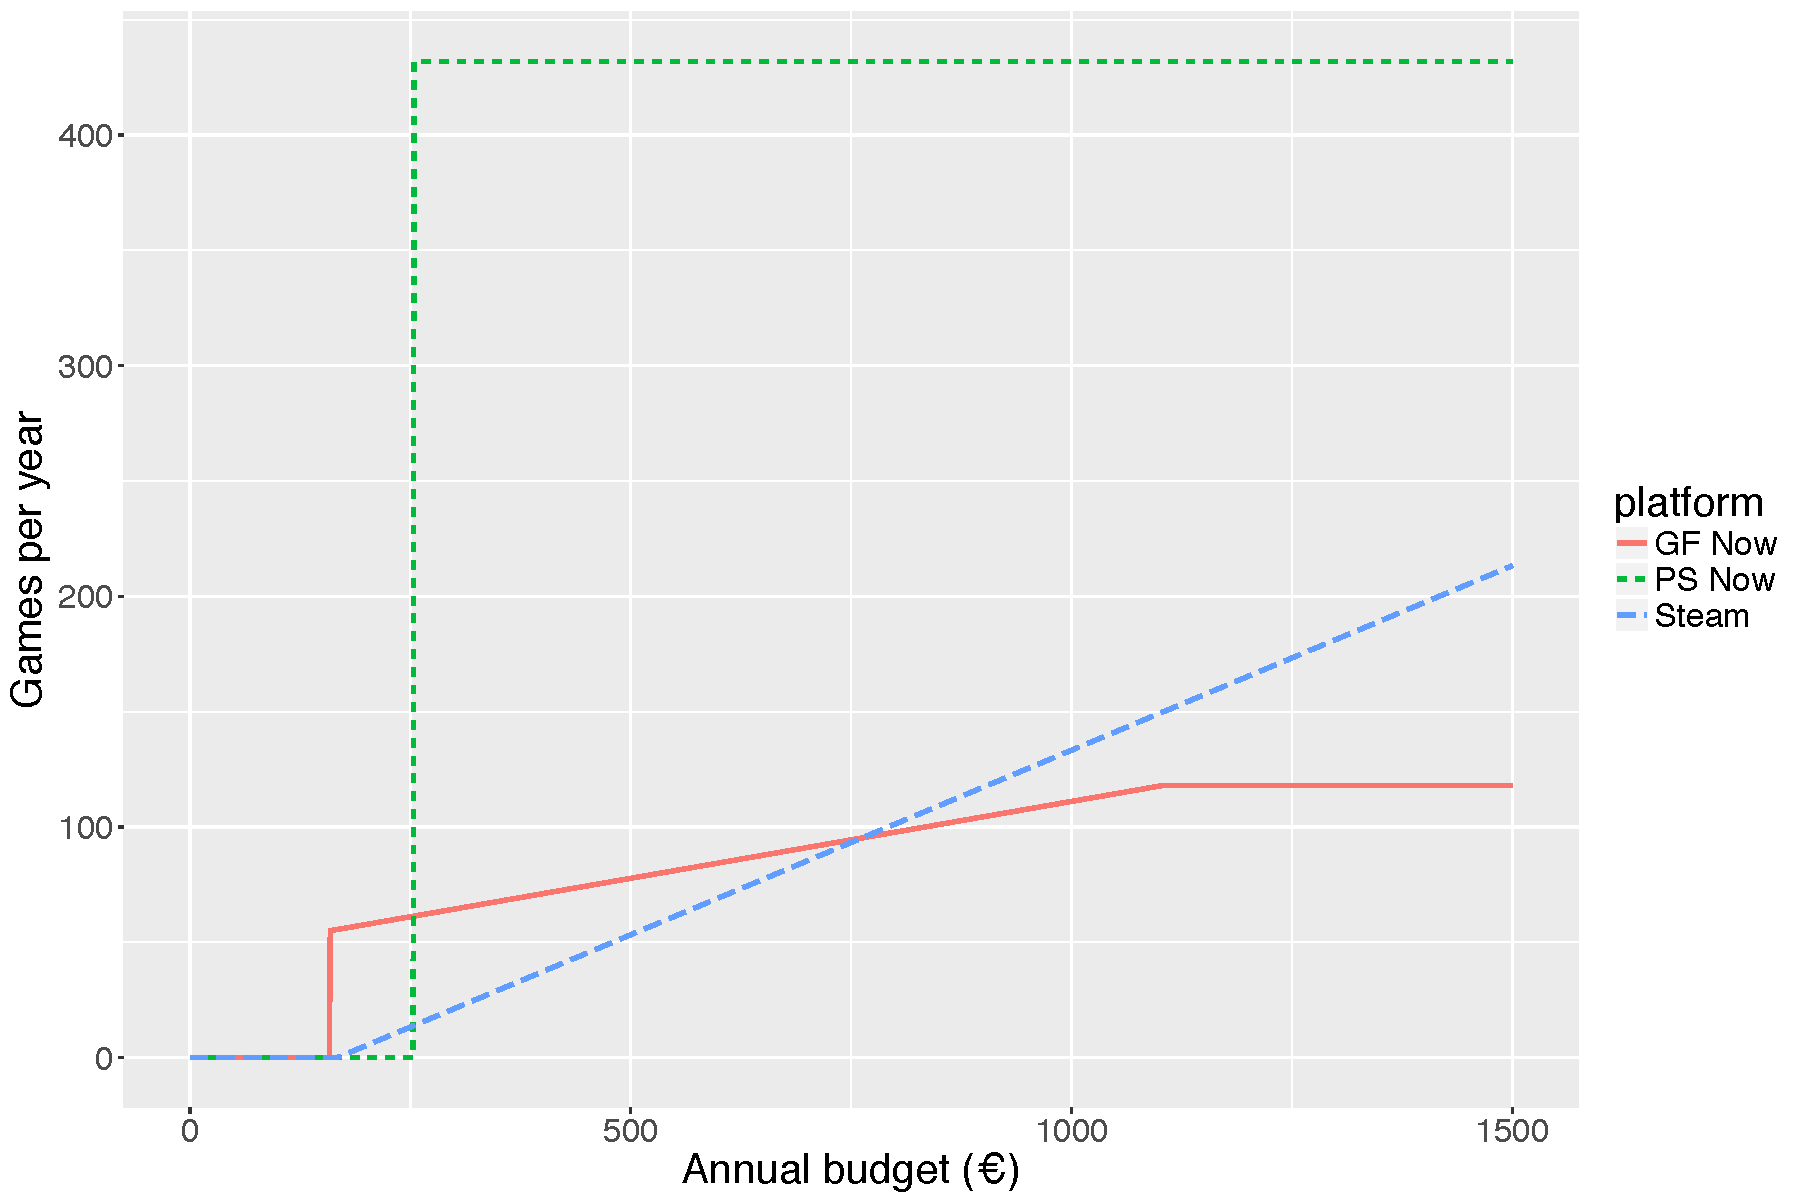
\includegraphics[width=1.0\columnwidth]{images/gamesperyear-over-budget.pdf}
	\caption{Affordable games per year on different platforms, given the customer's budget}
\label{fig:gamesperyear-over-budget}
\end{figure}


%%%%%%%%%%%%%%%%%%%%%%%%%%%%%%%%%%%%%%%%%%%
\paragraph{Affordable Games per Year Model}

The second model extends the previous one to span a period of multiple years, investigating the value one gets if a constant annual budget is spent. For the exemplary model, the budget is assumed to be $\text{\texteuro} 500$.
Figure~\ref{fig:games-over-years} depicts this example over ten years. On the two cloud platforms, the continual subscription costs limit the remaining budget for additional rental titles until the maximum number of titles is reached with that particular service, whereas the number of titles from \steam climbs steadily. The benefits of a multi-year commitment to these cloud gaming services therefore seem to be very limited, especially when considering that no games are retained after ending the subscription.

Increasing the annual budget further (to $\text{\texteuro} 1000$) exhausts the limited number of games on \psnow and \gfnow in or after the first year, respectively. Conversely, if only $\text{\texteuro} 260$ per year are available to spend on gaming, the cloud platforms' offers are larger than \steam's for four to six years.

\begin{figure}[!t]
	\centering
	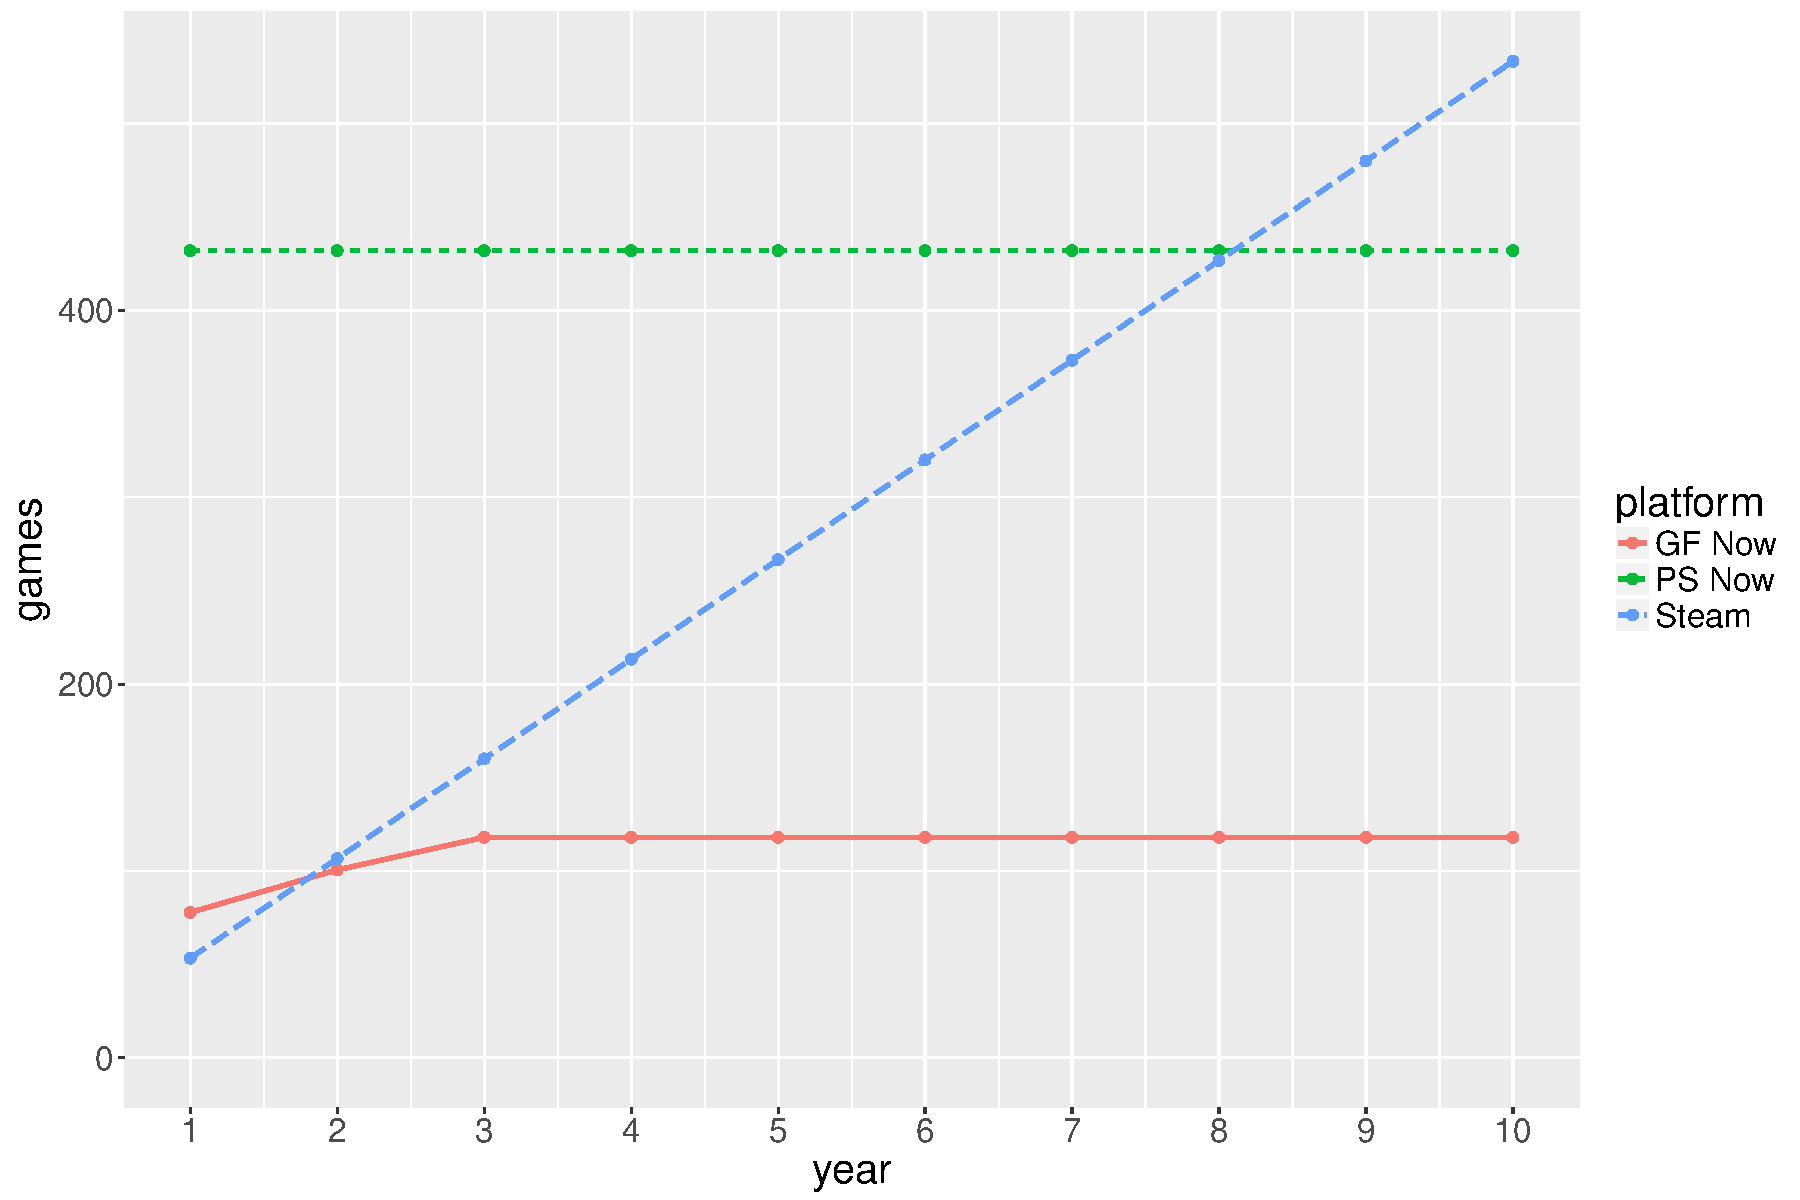
\includegraphics[width=1.0\columnwidth]{images/games-over-year.pdf}
	\caption{Number of affordable games per platform, assuming a yearly customer expenditure of $\text{\texteuro} 500$.}
\label{fig:games-over-years}
\end{figure}



%%%%%%%%%%%%%%%%%%%%%%%%%%%%%%%%%%%%%%%%%%%%%%%%%%%%%%%%%%%%%%%%%%%%%%%%%%%%%%%%
\subsection{Discussion}

This section mapped game and platform characteristics into simple user engagement metrics. For example, it is plausible that platforms with more, newer, and better-rated games attract more gamers; diversely distributed game lengths could be seen as catering to casual and dedicated gamer crowds likewise.
In terms of cost considerations, our models indicate that the current offers of \gfnow and \psnow best fit gamers on low budgets: Limitations on the amount of money that can be spent may somewhat mask the smaller range of offered games. If this is true, it further increases the economical pressure on cloud gaming platforms (as discussed in the following section). Overall, these investigations  expose the difference between an open market platform and the curated-by-necessity cloud gaming services.

%The size and sales-based price model of \steam poses challenges for direct competitors such as \gfnow. Services that cater to different audiences, such as \psnow which positions itself as a backwards compatibility service, may have more success in this regard. However, the limited target audience of \psnow becomes even narrower when the high subscription costs are taken into account, diminishing the benefits for many, not even considering the additional quality challenges that streaming video games brings along. All in all this may make curated Cloud Gaming services financially unattractive for the service's operator as is discussed in the following section.

% \todo[inline]{PZ: Ist Grafik \ref{fig:games-over-years} die Basis fuer die Steigung bei ps now usw. ab dem Eintritt in Fig.~\ref{fig:gamesperyear-over-budget}. Ps now wuerde ich als Club Good sehen.}
% \todo[inline]{FM: psnow/clubgood in the sense of a backwards compatibility service for devices that do not have native access to the streamed titles?.}

%PS Now specifically caters towards older titles and backwards compatibility, may find a niche here
% wer ist die zielgruppe?
% was ist die beste platform?
% gibt es eine mainstream platform?
% unterschiedliche ausrichtungen?





% metacritic titles:
% PC 16192
% PS4 817
% XB1 588
% WiiU 474
% 3DS 871
% GFNOW 68
% PSNOW 243
% STEAM 7749



% \begin{figure}[!t]
% 	\centering
% 	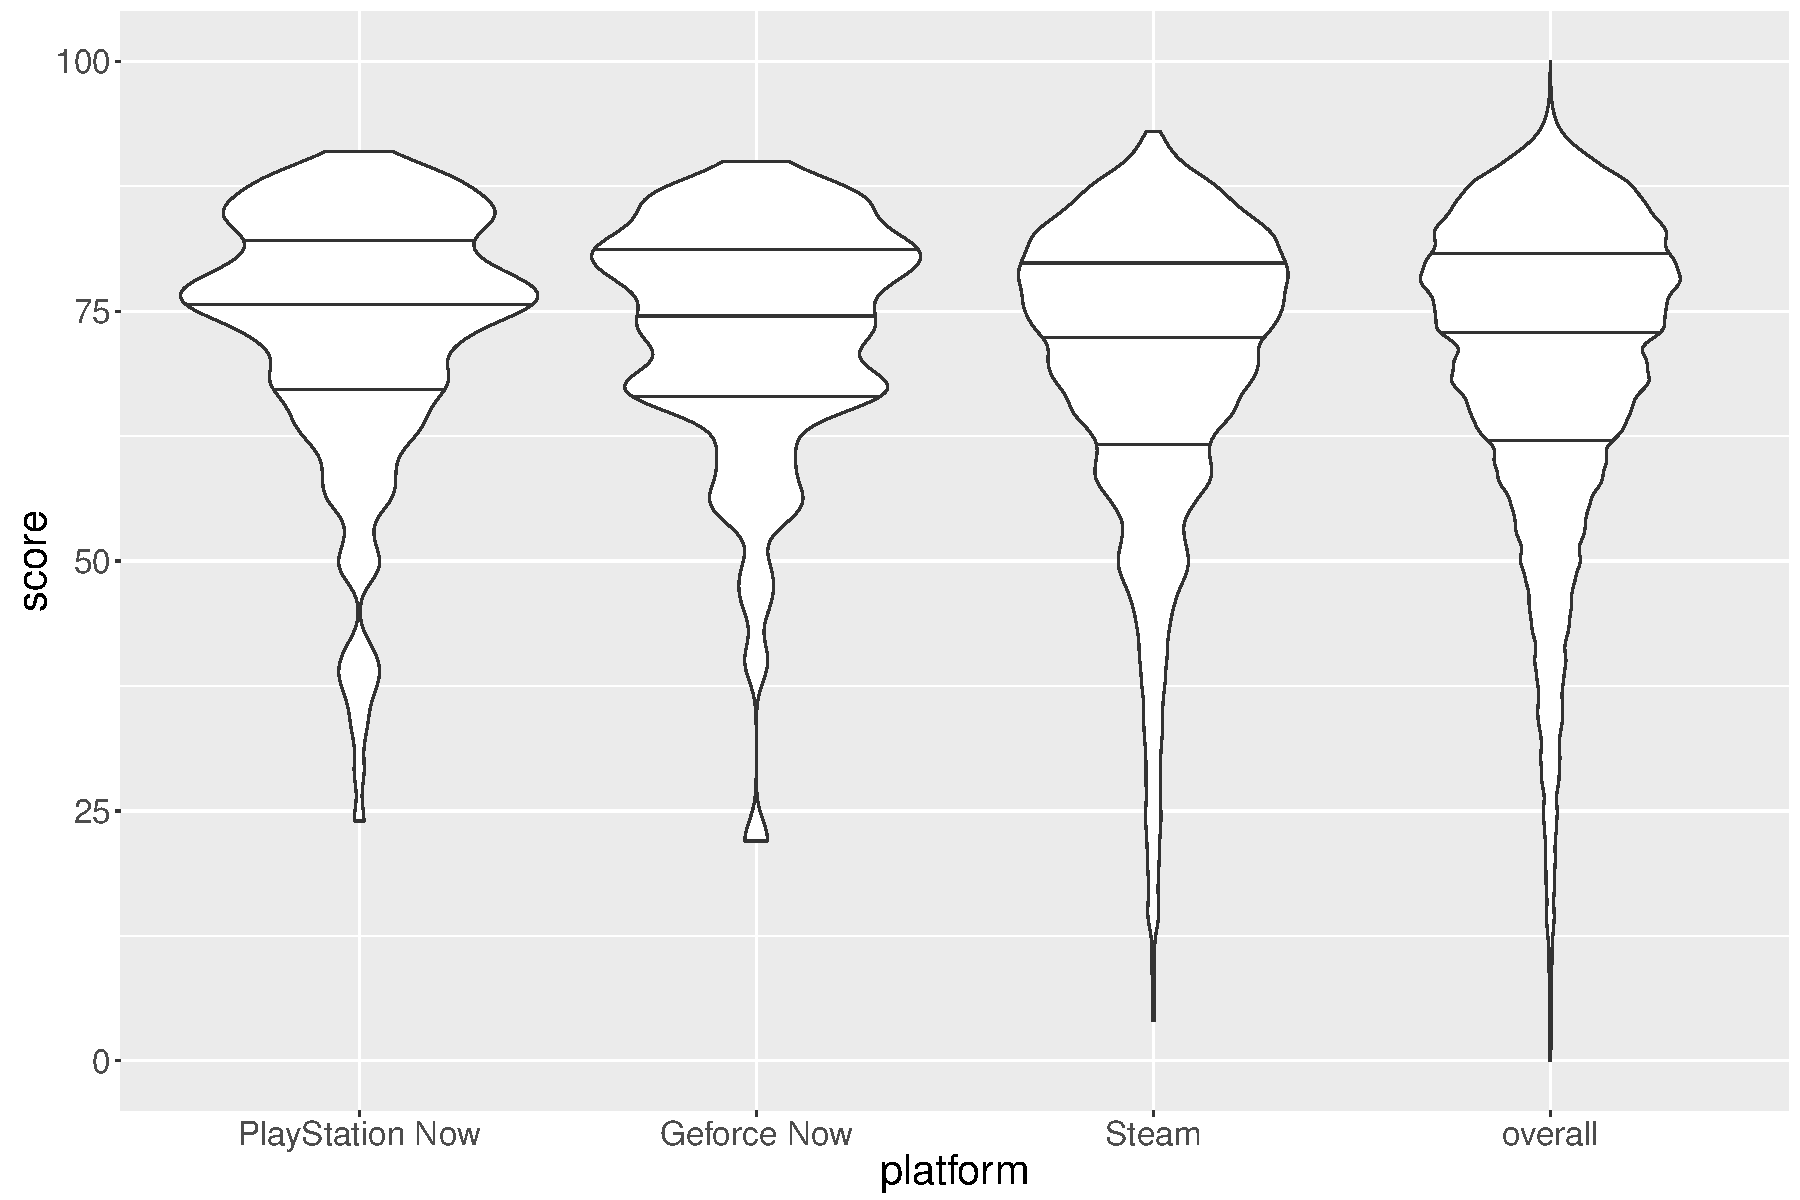
\includegraphics[width=1.0\columnwidth]{images/scores-by-platform-violin-userscore.pdf}
% 	\caption{Distribution of Metacritic user scores across the investigated platforms, depicted as violin plot with $25\%$, $50\%$, $75\%$ quantiles drawn.}
% \label{fig:userscores-by-platform}
% \end{figure}


% \subsection{E2E Lag}
% End-to-End Lag Model and Simulation in R. Now a standalone (submitted) paper at \url{https://github.com/mas-ude/onlinegame-lag-sim}. Can be referenced to argue the need for low E2E lag (meaning low network delay, but also the need for high fps).


%\item Graphical fidelity
%\item , tightness/precision/quality of controls and game mechanics, e2e lag
%\item Story?
%\item Other popularity measures? %(e.g. steamspy owner data?)
%\item Hardware requirements of games?
%\item Game costs and price history



% Caution: 
% Steam means game ownership
% PS/GF Now means only games during subscription plus permanent rental as long the sub is active(?)
% Additionally, PS Now means renting for 30 days